\documentclass[11pt, a4paper]{report}
\usepackage[utf8]{inputenc}
\usepackage{lscape}   % Make a page in landscape format \begin{landscape}
\usepackage{colortbl} % To color table cells
\usepackage{color} % Able to change textcolor
\usepackage[table]{xcolor}
\usepackage{longtable}
\usepackage{graphicx} % Able to add pictures
\usepackage{parskip}  % Separate paragraphs with a blank line
                      % rather than using indentation
\usepackage{hyperref} % Support for hyperlinks
\usepackage[protrusion=true,expansion=true]{microtype} % Improve justification
\usepackage{subfigure}
\usepackage{hyperref}
\usepackage{caption}
\usepackage{float}
\usepackage{afterpage}
\usepackage{lipsum}
\usepackage{wrapfig}
\usepackage{array}
\usepackage{sidecap}
\usepackage{appendix}
\usepackage{fancyhdr}
\usepackage{changepage}
\usepackage{tabularx}
\usepackage{multirow}


\hypersetup{%
    pdfborder = {0 0 0}
}

\begin{document}
	\begin{titlepage}
\begin{center}

{\Huge \bf Compendium} \\[1.0cm]
{\Huge \bf TDT4237 - Software Security}\\[1.0cm]
{\Large \bf Part one} \\

{\Large Security Engineering, second edition}

\vspace{14cm}

\centering
{\Large \bf By Marte Løge}



\end{center}
\end{titlepage}
	\clearpage 

	\tableofcontents

	\clearpage

	\chapter{What is Security Engeneering?}
\clearpage

{\bf A Framework} Good security engeneering requires four things to come together:
	\begin{enumerate} 
		\item {\bf Policy:} what you're supposed to achieve.
		\item {\bf Mechanism:} the chipers, access controls, hardware tamper-resistance
		and other mechinery that you assemblein order to implement the policy.
		\item {\bf Assurance:} the amount of reliance you can place on each particular mechanism.
		\item {\bf Incentive:} the motive that people guarding and maintaining the system
		have to do their job properly, and also the motive that the attackers have to try to defeat
		your policy. 
	\end{enumerate}


{\bf Why ae poor policy choices made? } Quite simply, the incentives on the decision makers
favor visible controls over effective ones. The result is what Bruce Schneier calls 
"security theatre" - measures designed to produce a feeling of security rather than the reality.


{\bf The role as a security engineer:} 
	\begin{itemize}
		\item We need to be able to put risks and threats in content.
		\item We need to be able to make realistic assessments of what might go wrong.
		\item We need to give our clients good advice.
	\end{itemize}


{\bf Case studies:} I will not describe these in detail. It is described in the book (pages 6-11).
	\begin{itemize}
		\item A bank
		\item A military base
		\item A hospital
		\item The Home
	\end{itemize}

\clearpage
\section{Definitions}
\subsection{System}
	\begin{enumerate}
		\item a product or component, such as a cryptographic protocol, a smartcard
		or the hardware of a PC.
		\item a collection of the above plus an operating system, communications and
		other things that go to make up an organization’s infrastructure.
		\item the above plus one or more applications (media player, browser, word
		processor, accounts / payroll package, and so on).
		\item any or all of the above plus IT staff.
		\item any or all of the above plus internal users and management;
		\item any or all of the above plus customers and other external users
	\end{enumerate}

\subsection{Subject, Person and Principal}
	\begin{itemize}
		\item{\bf Subject:} By a subject I will mean a physical person (human, ET, ...), 
		in any role including that of an operator, principal or victim. 
		\item{\bf Person:} By a person, I will mean either a physical person or a 
		legal person such as a company or government.
		\item{\bf Principal:} A principal is an entity that participates in a security system. 
		This entity can be a subject, a person, a role, or a piece of equipment such as a PC, smartcard, or
		card reader terminal. A principal can also be a communications channel (which
		might be a port number, or a crypto key, depending on the circumstance). A
		principal can also be a compound of other principals
	\end{itemize}

\subsection{Identity} 

\clearpage
\subsection{Trust and Trustworthy} 
	The definitions of trust and trustworthy are often confused. 
	The following example illustrates the difference: if an NSA employee is observed in a toilet
	stall at Baltimore Washington International airport selling key material to a
	Chinese diplomat, then (assuming his operation was not authorized) we can
	describe him as ‘trusted but not trustworthy’. Hereafter, we’ll use the NSA
	definition that a trusted system or component is one whose failure can break the
	security policy, while a trustworthy system or component is one that won’t fail.

\subsection{Confidenciality, Privacy and Secrecy}
	\begin{itemize}
		\item {\bf Secrecy} is a technical term which refers to the effect of the mechanisms
		used to limit the number of principals who can access information, such
		as cryptography or computer access controls.
		\item {\bf Confidentiality} involves an obligation to protect some other person’s 
		or organization’s secrets if you know them.
		\item {\bf Privacy} is the ability and/or right to protect your personal information
		and extends to the ability and/or right to prevent invasions of personal space.
	\end{itemize}

\subsection{Authenticity and Integrity}


\clearpage
\section*{Summary}
\begin{itemize}
	\item Framework
	\item Security theatre
	\item The role as a security engineer
	\item Case studies (bank, military base, hospital, the Home)
	\item Definition: System
	\item Definitions: subject, person and principal
	\item Identity
	\item Trust and Trustworthy
	\item Confidenciality, Privacy and Secrecy
	\item Authenticity and Integrity
\end{itemize}

 
	\clearpage
	\chapter{Usability and Psychology}

{\bf Social engineering}

\clearpage
\section{Attacks Based on Psychology}

	\subsection{Pretexting}
	Pretexting is a form of social engineering in which an individual lies to obtain privileged data. 
	A pretext is a false motive. Pretexting often involves a scam where the liar pretends to need 
	information in order to confirm the identity of the person he is talking to. After establishing 
	trust with the targeted individual, the pretexter might ask a series of questions designed to 
	gather key individual identifiers.

	The pretexter's goal is to obtain personal information about you, such as your SSN, your bank or 
	credit card account numbers, mother's maiden name, information contained in your credit report, 
	or the existence and size of your savings and investment portfolios.
	After getting your answers, the pretexter may call your financial institution pretending to 
	be you or someone with authorized access to your account. The pretexter may, for example, 
	claim that he's forgotten his checkbook and needs information about his account.

	\begin{figure}[H]
		
\includegraphics[width=\textwidth]{pics/pretexting.png}
	\end{figure}

	\clearpage
	\subsection{Phising}
	Phishing is a technique of fraudulently obtaining private information. Typically, the phisher sends 
	an e-mail that appears to come from a legitimate business — a bank, or credit card company—requesting
	"verification" of information and warning of some dire consequence if it is not provided. The e-mail 
	usually contains a link to a fraudulent web page that seems legitimate — with company logos and content
	and has a form requesting everything from a home address to an ATM card's PIN.

	\begin{figure}[H]
		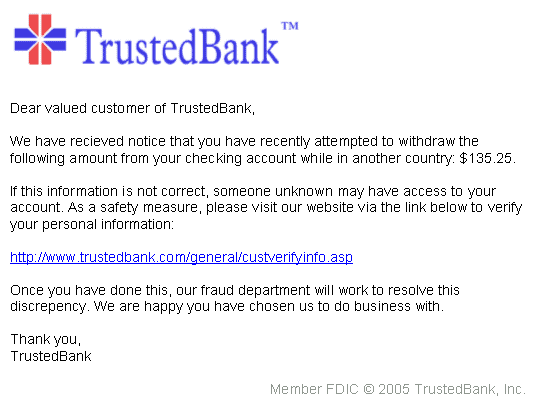
\includegraphics[width=\textwidth]{pics/phishing.png}
		\caption{Phising attempt}
	\end{figure}

\clearpage
\section{Insights from Psychology Research}
	
	\subsection*{What the Brain does Worse Than the Computer}
	\begin{itemize}
		\item Actions performed often become a matter of skill, but this comes with
		a downside: inattention can cause a practised action to be performed
		instead of an intended one. We are all familiar with such capture errors;
		an example is when you intend to go to the supermarket on the way home from 
		work but take the road home by mistake — as that’s what you do most days. 
		In computer systems, people are trained to click ‘OK’ to pop-up boxes as that’s 
		often the only way to get the work done; some attacks have used the fact that 
		enough people will do this even when they know they shouldn’t.
		\item Actions that people take by following rules are open to errors when 
		they follow the wrong rule. Various circumstances — such as information overload 
		— can cause people to follow the strongest rule they know, or the most general rule, 
		rather than the best one. Examples of phishermen getting people to follow the wrong 
		rule include using https (because ‘it’s secure’) and starting URLs with the 
		impersonated bank’s name, as www.citibank.secureauthentication.com — 
		looking for the name being for many people a stronger rule than parsing its position.
		\item The third category of mistakes are those made by people for cognitive
		reasons — they simply don’t understand the problem. For example, Microsoft’s latest 
		(IE7) anti-phishing toolbar is easily defeated by a picture-in-picture attack. 
	\end{itemize}

	\begin{figure}[H]
		\centering
		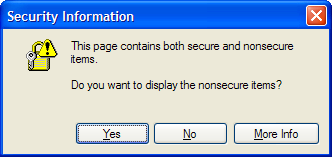
\includegraphics[scale=0.8]{pics/insecureweb.png}
		\caption{Actions performed often become a matter of skill}
	\end{figure}

	\clearpage
	\subsection*{Preceptual Bias and Behavioural Economics}
		\begin{itemize}
			\item How do people make decisions faced with uncertainty?
			\item By framing an action as a gain rather than as a loss makes people more 
			likely to take it. 
			\item We’re also bad at calculating probabilities, and use all sorts of heuristics 
			to help us make decisions: we base inferences on familiar or easily-imagined analogies, 
			and by comparison with recent experiences.
			\item We also worry too much about unlikely events. We’re morelikely to be sceptical 
			about things we’ve heard than about things we’ve seen.
			\item Many frauds work by appealing to our atavistic instincts to trust people 
			more in certain situations or over certain types of decision.
			\item Many people perceive terrorism to be a much worse threat than food poisoning 
			or road traffic accidents: this is irrational.
			We overestimate the small risk of dying in a terrorist attack not just 
			because it’s small but because of the visual effect of the 9/11 on TV.
			\item Global warming doesn’t violate anyone’s moral sensibilities and
			it’s a long-term threat rather than a clear and present danger. Humans are 
			sensitive to rapid changes in the environment rather than slow ones.
			\item We are less afraid when we’re in control, such as when driving a car, as opposed 
			to being a passenger in a car or airplane and we are more afraid of 
			uncertainty, that is, when the magnitude of the risk is unknown.
			\item We have a tendency to plump for the alternative that’s ‘good enough’ rather than 
			face the cognitive strain of trying to work out the odds perfectly. Another
			aspect of this is that many people just plump for the standard configuration
			of a system, as they assume it will be good enough. This is one reason why
			secure defaults matter.
			\item The appearance of protection can matter just as much as the reality. For example,
			many people don't use electronic banking because of a fear of fraud, so banks pay
			a fortune for the time of branch and call-center staff. It's not enough for the security engineer to stop bad things happening; you also have to reassure people.
		\end{itemize} 

		\begin{figure}[H]
			\centering
			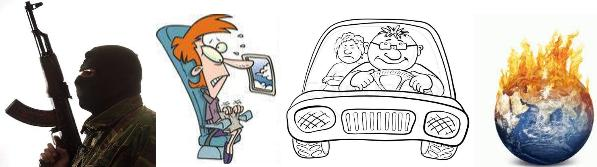
\includegraphics[scale=0.5]{pics/uncertainty.jpg}
		\end{figure}

	\subsection*{Differences Between People - Gender}
		Most information systems are designed by men, and yet over half their
		users may be women. Recently people have realised that software can create
		barriers to females, and this has led to research work on ‘gender HCI’ — on
		how software should be designed so that women as well as men can use
		it effectively. For example, it’s known that women navigate differently from
		men in the real world, using peripheral vision more, and it duly turns
		out that larger displays reduce gender bias. Other work has focused on
		female programmers, especially end-user programmers working with tools
		like spreadsheets. It turns out that women tinker less than males, but more
		effectively. 

		Women appear to be more thoughtful, but lower self-esteem and
		higher risk-aversion leads them to use fewer features. Given that many of the
		world’s spreadsheet users are women, this work has significant implications
		for product design.

		Simon Baron-Cohen, classifies human brains into type S (systematizers) and 
		type E (empathizers). Type S people are better at geometry and some 
		kinds of symbolic reasoning, while type E's are better at language and 
		multiprocessing. Most men are type S, while most women are type E, a 
		relationship that Baron-Cohen believes is due to
		fetal testosterone levels. 

		\begin{figure}[H]
			\centering
			
\includegraphics[scale=0.4]{pics/gender.jpg}
			\caption{Are security mechanisms gender-neutral?}
		\end{figure}

	\clearpage
	\subsection*{Social Psychology}
		This discipline attempts to explain how the thoughts, feelings, and behaviour
		of individuals are influenced by the actual, imagined, or implied presence of
		others. It has many aspects, from the identity that people derive from belonging
		to groups, through the self-esteem we get by comparing ourselves with others.

		The growth of social-networking systems will
		lead to peer pressure being used as a tool for deception, just as it is currently
		used as a tool for marketing fashions.

		Experiments has showed that people will obey an authority rather than their conscience. 
		Most people will do downright immoral things if they are told to.
		A Experiment showed that normal people can behave wickedly even in the absence of orders. 
		In 1971, experimenter Philip Zimbardo set up a ‘prison’ at Stanford where 24 students
		were assigned at random to the roles of 12 warders and 12 inmates. The aim
		of the experiment was to discover whether prison abuses occurred because
		warders (and possibly prisoners) were self-selecting. However, the students
		playing the role of warders rapidly became sadistic authoritarians.
		Abuse of authority, whether real or ostensible, is a major issue for people
		designing operational security measures. Abuse of authority are the key in 
		in security experiments. 

	\begin{figure}[H]
		\centering
		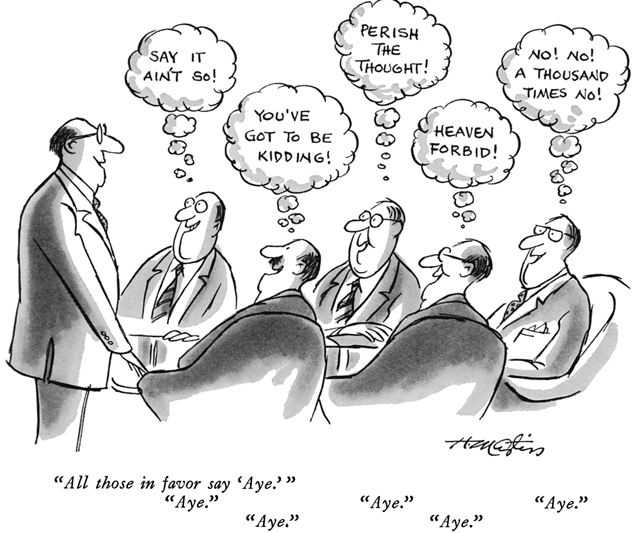
\includegraphics[scale=0.5]{pics/authority.png}
	\end{figure}


	\subsection*{What the Brain Does Better Than the Computer}
		\begin{itemize}
			\item We are extremely good at recognising other humans visually, an ability shared by 
			many primates.
		
			\item We are good at image recognition generally; a task such as ‘pick out all scenes
			in this movie where a girl rides a horse next to water’ is trivial for a human
			child yet a hard research problem in image processing. 

			\item We’re also better thanmachines at understanding speech, particularly in noisy 
			environments, and at identifying speakers.

			\item These abilities mean that it’s possible to devise tests that are easy for humans
			to pass but hard for machines — the so-called ‘CAPTCHA’ test.
		\end{itemize}

\clearpage
\section{Passwords}

	It’s hard to think of a worse authentication mechanism than passwords, given
	what we know about human memory: people can’t remember infrequently-
	used, frequently-changed, or many similar items; we can’t forget on demand;
	recall is harder than recognition; and non-meaningful words are more difficult.

	There are system and policy issues too: as people become principals in more
	and more electronic systems, the same passwords get used over and over
	again. Not only may attacks be carried out by outsiders guessing passwords,
	but by insiders in other systems. People are now asked to choose passwords
	for a large number of websites that they visit rarely.

	Passwords are not, of course, the only way of authenticating users to
	systems. There are basically three options. The person may retain physical
	control of the device — as with a remote car door key. The second is that
	she presents something she knows, such as a password. The third is to use
	something like a fingerprint or iris pattern
	
	Passwords matter, and managing them is a serious real world problem
	that mixes issues of psychology with technical issues. There are basically three
	broad concerns, in ascending order of importance and difficulty:
	
		\begin{enumerate}
			\item Will the user enter the password correctly with a high enough
			probability?
			\item Will the user remember the password, or will they have to either write it
			down or choose one that’s easy for the attacker to guess?
			\item Will the user break the system security by disclosing the password
			to a third party, whether accidentally, on purpose, or as a result of
			deception?
		\end{enumerate}


\clearpage
\subsection{Difficulties with Remembering the Password}

	Our first human-factors issue is that if a password is too long or complex,
	users might have difficulty entering it correctly.

	when customers are expected to memorize passwords, they either choose values which are easy for
	attackers to guess, or write them down, or both. In fact, the password problem
	has been neatly summed up as: ‘‘Choose a password you can’t remember, and
	don’t write it down.’’

	People choose naive passwords. People will use names, single letters, or even just hit carriage return
	giving an empty string as their password. So some systems started to require
	minimum password lengths, or even check user entered passwords against a
	dictionary of bad choices. However, password quality enforcement is harder
	than you might think. 



\subsection{User Abilities, Training and Design Errors}
	So what can you realistically expect from users when it comes to
	choosing and remembering passwords?

	After a experiment (page 35-36) on password an humans, the conclusion was:
	\begin{itemize}
		\item For users who follow instructions, passwords based on mnemonic
		phrases offer the best of both worlds. They are as easy to remember as
		naively selected passwords, and as hard to guess as random passwords.
		\item The problem then becomes one of user compliance. A significant number
		of users (perhaps a third of them) just don’t do what they’re told.
	\end{itemize}

	An important example of how not to do it is to ask for ‘your mother’s
	maiden name’. A surprising number of banks, government departments and
	other organisations authenticate their customers in this way. But there are two
	rather obvious problems. First, your mother’s maiden name is easy for a thief
	to find out, whether by asking around or using online genealogical databases.
	Second, asking for a maiden name makes assumptions which don’t hold for
	all cultures, so you can end up accused of discrimination: Icelanders have no
	surnames, and women from many other countries don’t change their names
	on marriage. Third, there is often no provision for changing ‘your mother’s
	maiden name’, so if it ever becomes known to a thief your customer would
	have to close bank accounts (and presumably reopen them elsewhere). 

	A general error is failing to reset the default password in systems. 
	Often is the default password the same in many different systems!

	Banks have put som effort into trying to train their customers to look 
	for certain features in websites: check the english, look for the lock symbol, 
	it is ok to click on images, but not on URL's, hover your mouse over links 
	before clicking on it, etc. This sort of arms race is more likely to benefit
	the attackers because the customers get very predictable in how they act.

\subsection{Social-Engineering Attacks}

	‘This is the security department of your bank. We see that your card
	has been used fraudulently to buy gold coins. I wonder if you can tell me the
	PIN, so I can get into the computer and cancel it?’. This even works by email!

	A huge problem is that many banks and other businesses train their customers to act in
	unsafe ways. It’s not prudent to click on links in emails, so if you want to
	contact your bank you should type in the URL or use a bookmark — yet bank
	marketing departments continue to send out emails containing clickable links.
	Many email clients — including Apple’s, Microsoft’s, and Google’s — make
	plaintext URLs clickable, and indeed their users may never see a URL that
	isn’t. This makes it harder for banks to do the right thing.

	If even the fraud department doesn’t understand that banks ought to be able to 
	identify themselves, and that customers should not be trained to give out 
	security information on the phone, what hope is there? When even a bank’s 
	security department can’t tell spam from phish, how are their customers supposed to?

	\clearpage
	{\bf Trusted Path:} A thread in the background of phishing is trusted path, 
	which refers to some means of being sure that you’re logging into a genuine machine
	through a channel that isn’t open to eavesdropping. Here the deception is
	more technical than psychological; rather than inveigling a bank customer into
	revealing her PIN to you by claiming to be a policeman, you steal her PIN
	directly by putting a false ATM in a shopping mall. A public
	terminal would be left running an attack program that looks just like the usual
	logon screen — asking for a user name and password. When an unsuspecting
	user does this, it will save the password somewhere in the system, reply
	‘sorry, wrong password’ and then vanish, invoking the genuine password
	program. The user will assume that he made a typing error first time and
	think no more of it. 

	Have you wondered why Windows have the anoying ctrl-alt-del part befor login?
	It is there to make sure you will be entering genuine password prompt.

	Other similar attacks is mofifoed keyboard, keyloggers, and skimmed bank terminals.
	I sometimes wonder, what if there is a keylogger in a windows system?
	If you press ctrl-alt-del, you will simply tell the attacker where your password is.
	The logged txt file will then have something like "ctrl alt del username password".

	Two-factor authentication is now widley used. The basic idea is that it consists
	of something you have and something you know. It will be described in later chapters. 

\clearpage
\section{System Issues}

	There are also technical issues to do with password entry and storage that will 
	be briefly covered here. Here are some examples of attacks we are trying to defend against:

	\begin{itemize}
		\item Targeted attack on one account (when sending email it is known as spear phishing)
		\item Attempt to penetrate any account on a system
		\item Service denial attack
	\end{itemize}

	{\bf Can you deny service?} Banks often have a rule that a terminal and user account
	are frozen after three bad password attempts; after that, an administrator has to 
	reactivate them. It sure works in a website, but what in the military? Could a system
	like this benefit the enemy/attacker? Many commercial websites nowadays don't limit guessing
	becuase of the possibility of such an attack (service denial attack).

	{\bf Interface design: } I usually cover my dialling hand with my body or my other hand when
	entering a card number or PIN in a public place — but you shouldn’t design
	systems on the assumption that all your customers will do this. Many people
	are uncomfortable shielding a PIN from others as it’s a visible signal of distrust.
	Because of this, a targeted attack against a person could be easy!

	{\bf Eavesdropping: } The latest modus operandi is for bad people
	to offer free WiFi access in public places, and harvest the passwords that
	users enter into websites. This is a kind of attempt to just get all sensitive information
	about anyone, and not just a specific person. 

	{\bf Timing attack: }Many kids find out that a bicycle combination lock can usually be 
	broken in a few minutes by solving each ring in order of looseness. The same idea
	worked against a number of computer systems. The PDP-10 TENEX operating
	system checked passwords one character at a time, and stopped as soon as
	one of them was wrong. This opened up a timing attack: the attacker would
	repeatedly place a guessed password in memory at a suitable location, have it
	verified as part of a file access request, and wait to see how long it took to be
	rejected


	{\bf Car keys (fail):} Have you ever heard a story about someone that could open 
	many cars at a parking lot with their own key? Yes, this is a kind of system fails
	where the number of bits used for opening a car was to small in order of how many
	cars that needed an uniqe key.

	{\bf One-way encryption and plaintext storage:} Password storage has also been a problem 
	for some systems. Keeping a plaintext file of passwords can be dangerous. The best way
	of storing a password is password + salt + hashing (can also add pepper to it).

	{\bf Prevent more than x attempts or log all attempts? }

	There are various problems with this doctrine, of which the worst may be that 
	the attacker’s goal is often not to guess some particular user’s password 
	but to get access to any account. If a large defense network has a million 
	possible passwords and a million users, and the alarm goes off after three 
	bad password attempts on any account, then the attack is to try one password 
	for every single account. Thus the quantity of real interest is the probability 
	that the password space can be exhausted in the lifetime of the system at the 
	maximum feasible password guess rate.

	To prevent more than one password guess every few seconds per user account, or 
	(if you can) by source IP address. You might also keep a count of all the failed 
	logon attempts and analyse them: is there a constant series of guesses that could 
	indicate an attempted intrusion? (And what would you do if you noticed one?).

\section{CAPTCHA's}

	Recently people have tried to design protection mechanisms that use the
	brain’s strengths rather than its weaknesses. One early attempt was Passfaces:
	this is an authentication system that presents users with nine faces, only one
	of which is of a person they know; they have to pick the right face several
	times in a row to log on [356]. The rationale is that people are very good
	at recognising other people’s faces, but very bad at describing them: so you
	could build a system where it was all but impossible for people to give away
	their passwords, whether by accident or on purpose. Other proposals of this
	general type have people selecting a series of points on an image — again,
	easy to remember but hard to disclose. Both types of system make shoulder
	surfing harder, as well as deliberate disclosure offline.

	The most successful innovation in this field, however, is the CAPTCHA —
	which stands for ‘Completely Automated Public Turing Test to Tell Computers
	and Humans Apart.’

	The idea is that a program generates some random text,
	and produces a distorted version of it that the user must decipher. Humans
	are good at reading distorted text, while programs are less good. 

	It is inspired by the test famously posed by Alan Turing as to whether a computer
	was intelligent, where you put a computer in one room and a human in
	another, and invite a human to try to tell them apart. 


	\clearpage
	\chapter{Protocols}

\clearpage
\section{Password Eavesdropping Risks}
A good case study comes from simple embedded systems, such as the remote control used to open
your garage or to unlock the doors of cars manufactured up to the mid-1990’s.
These primitive remote controls just broadcast their serial number, which also
acts as the password. An attack that became common was to use a ‘grabber’, a device 
that would record a code broadcast locally and replay it later. 

sixteen-bit passwords are too short. It occasionally happened that people found they could unlock 
the wrong car by mistake. By the mid-1990’s, devices appeared which could try all
possible codes one after the other. A code will be found on average after about
215 tries, which at ten per second takes under an hour. A thief operating in a
parking lot with a hundred vehicles within range would be rewarded in less
than a minute with a car helpfully flashing its lights.



\section{Simple Authentication}

	{\bf Nonce:} The term nonce can mean anything that guarantees the freshness of a
	message. A nonce can, according to the context, be a random number, a serial
	number, a random challenge received from a third party, or even a timestamp.

	{\bf Security and business: } Security mechanisms are used more and more to support business 
	models, by accessory control, rights management, product tying and bundling. It is
	wrong to assume blindly that security protocols exist to keep ‘bad’ guys ‘out’.
	They are increasingly used to constrain the lawful owner of the equipment in
	which they are built; their purpose may be of questionable legality or contrary
	to public policy. For example: Many printer companies embed authentication mechanisms 
	in printers to ensure that genuine toner cartridges are used. If a competitor’s 
	product is loaded instead, the printer may quietly downgrade from 1200 dpi to 300 dpi, 
	or simply refuse to work at all. Mobile phone vendors make a lot of money from 
	replacement batteries, and now use authentication protocols to spot competitors’ 
	products so they can be blocked or even drained more quickly. 

	\clearpage
	\subsection{Challenge and response}

		Many cars use a more sophisticated two-pass protocol, called challenge-response, 
		to actually authorise engine start. As the car key is inserted into the steering lock, 
		the engine controller sends a challenge consisting of a random n-bit number to the key 
		using short-range radio. The car key computes a response by encrypting the challenge. 
		This is still not bulletproof, how random is random?

		{\bf two-factor authentication:} A much more visible use of challenge-response is in two-factor authentication.
		Many organizations issue their staff with password generators to let them
		log on to corporate computer systems. These may look like calculators
		but their main function is as follows; when you want to log in to a machine on the network, 
		you call up a logon screen and are presented with a random challenge of maybe seven digits. 
		You key this into your password generator, together with a PIN of maybe four
		digits. The device encrypts these eleven digits using a secret key shared with
		the corporate security server, and displays the first seven digits of the result.
		You enter these seven digits as your password.

	\subsection{Reflection Attacks}
		--Write something here?--

\clearpage
\section{Manipulating the Message}

	An example is when dishonest cabbies insert pulse generators in the cable
	that connects their taximeter to a sensor in their taxi’s gearbox. The sensor
	sends pulses as the prop shaft turns, which lets the meter work out how far
	the taxi has gone. A pirate device, which inserts extra pulses, makes the taxi
	appear to have gone further. 

	Another example is a key log attack which defeated many pay-TV systems. 
	If the messages that pass between the smartcard and the decoder are the same for
	all decoders (which is usually the case) then a subscriber can log all the keys
	sent by his card to his decoder and post it online somewhere. People without a
	subscription, but who have video-recorded the enciphered program, can then
	download the key log and use it to decipher the tape.

	
\section{Changing the Environment}

	A very common cause of protocol failure is that the environment changes, so
	that assumptions which were originally true no longer hold and the security
	protocols cannot cope with the new threats.

	For example, a passenger who commuted a long distance from a suburban station 
	to downtown might buy two cheaper, short distance season tickets — one between 
	his suburban station and a nearby one, and the other between his destination 
	and another downtown station. 

	An other example is a one-day travel pass in London.
	When a one-day travel pass was sold, the revenue was distributed between 
	the various bus, train and subway operators using a formula that depended on where it 
	was sold. Suddenly, the train companies had a motive to book all their ticket sales 
	through the outlet that let them keep the largest percentage. As well as bad outsiders
	(passengers), we now had bad insiders (rail companies), and the design just
	hadn’t allowed for them. Chaos and litigation ensued.

	The transport system’s problem was not new; it had been observed in the
	Italian ski resort of Val di Fassa in the mid-1970’s. There, one could buy a
	monthly pass for all the ski lifts in the valley. An attendant at one of the lifts
	was observed with a deck of cards, one of which he swiped through the reader
	between each of the guests. It turned out that the revenue was divided up
	between the various lift operators according to the number of people who had
	passed their turnstiles. So each operator sought to inflate its own figures as
	much as it could.


\section{Chosen Protocol Attacks}
	Here’s one example. It used to be common for people visiting a porn
	website to be asked for ‘proof of age,’ which usually involves giving a
	credit card number, whether to the site itself or to an age checking service.
	If credit and debit cards become usable in PCs, it would be natural for
	the porn site to ask the customer to authenticate a random challenge as
	proof of age. A porn site can then mount a ‘Mafia-in-the-middle’ attack. 
	They wait until an unsuspecting customer visits their site,
	then order something resellable (such as gold coins) from a dealer, playing
	the role of the coin dealer’s customer. When the coin dealer sends them the
	transaction data for authentication, they relay it through their porn site to
	the waiting customer. The poor man OKs it, the Mafia gets the gold coins, and
	when thousands of people suddenly complain about the huge charges to their
	cards at the end of the month, the porn site has vanished — along with the
	gold. 


\section{Managing Encryption Keys}

	Authentication protocols are now also used in distributed computer systems
	for general key management purposes, and are therefore becoming ever more
	important. Kerberos was the first such system to come into widespread use,
	and a variant of it is used in Windows. 

	\subsection{Basic Key Management}
		The basic idea behind key distribution protocols is that where two princi-
		pals want to communicate, they may use a trusted third party to effect an
		introduction.
		When discussing authentication protocols, it is conventional to give the
		principals human names in order to avoid getting lost in too much algebraic
		notation. So we will call the two communicating principals {\bf ‘Alice’} and 
		{\bf ‘Bob’}, and the trusted third party {\bf ‘Sam’}. 

		A simple authentication protocol could run as follows.
		\begin{enumerate}
			\item Alice first calls Sam and asks for a key for communicating with Bob.
			\item Sam responds by sending Alice a pair of certificates. Each contains a copy
			of a key, the first encrypted so only Alice can read it, and the second
			encrypted so only Bob can read it.
			\item Alice then calls Bob and presents the second certificate as her introduction.
			Each of them decrypts the appropriate certificate under the key they share
			with Sam and thereby gets access to the new key. Alice can now use the
			key to send encrypted messages to Bob, and to receive messages from him
			in return.
		\end{enumerate}

		\begin{figure}[H]
			\centering
			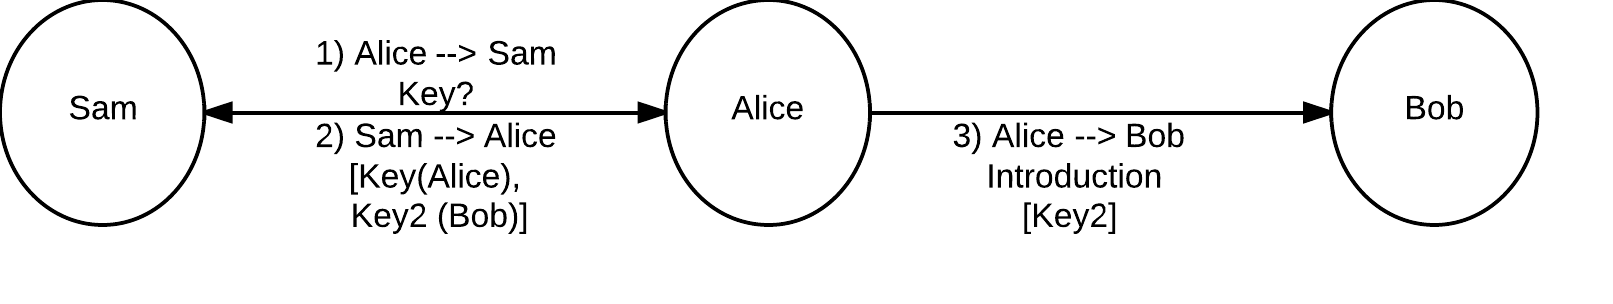
\includegraphics[scale=0.20]{pics/BobAliceSam1.png}
		\end{figure}

		Expanding the notation, Alice calls Sam and says she’d like to talk to
		Bob. Sam makes up a session key message consisting of Alice’s name, Bob’s
		name, a key for them to use, and a timestamp. He encrypts all this under
		the key he shares with Alice, and he encrypts another copy of it under the
		key he shares with Bob. He gives both ciphertexts to Alice. Alice retrieves
		the key from the ciphertext that was encrypted to her, and passes on to
		Bob the ciphertext encrypted for him. She now sends him whatever message
		she wanted to send, encrypted using this key.
		Replay attacks are a known problem with authentication protocols, so in
		order that both Bob and Alice can check that the certificates are fresh, Sam may
		include a timestamp in each of them. If certificates never expire, there might
		be serious problems dealing with users whose privileges have been revoked.

		\begin{figure}[H]
			\centering
			
\includegraphics[scale=0.5]{pics/basicKeyManagement.png}
		\end{figure}

	\subsection{The Needham-Schroeder Protocol}
		Many existing key distribution protocols are derived from the Needham-Schroeder
		protocol, which appeared in 1978 [960]. It is somewhat similar to the above,
		but uses nonces rather than timestamps. It runs as follows:

		\begin{figure}[H]
			\centering
			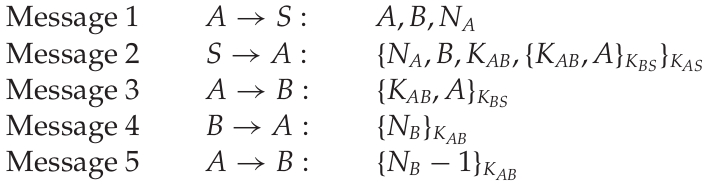
\includegraphics[scale=0.4]{pics/NeedhamSchroederProtocol.png}
		\end{figure}

		Here Alice takes the initiative, and tells Sam: ‘I’m Alice, I want to talk to Bob,
		and my random nonce is NA .’ Sam provides her with a session key, encrypted
		using the key she shares with him. This ciphertext also contains her nonce so
		she can confirm it’s not a replay. He also gives her a certificate to convey this
		key to Bob. She passes it to Bob, who then does a challenge-response to check
		that she is present and alert.

		There is a subtle problem with this protocol — Bob has to assume that the
		key KAB he receives from Sam (via Alice) is fresh. This is not necessarily so.

	\subsection{Kerberos}
		An important practical derivative of the Needham-Schroeder protocol may be
		found in Kerberos, a distributed access control system that originated at MIT
		and is now one of the standard authentication tools in Windows. Instead
		of a single trusted third party, Kerberos has two kinds: an authentication server
		to which users log on, and a ticket granting server which gives them tickets
		allowing access to various resources such as files. This enables more scalable
		access management. In a university, for example, one might manage students
		through their halls of residence but manage file servers by departments; in
		a company, the personnel people might register users to the payroll system
		while departmental administrators manage resources such as servers and
		printers.

		\begin{figure}[H]
			\centering
			
\includegraphics[scale=0.5]{pics/Kerberos.png}
		\end{figure}
		
		Translating this into English: Alice asks the ticket granting server for access
		to B. If this is permissible, the ticket {TS , L, KAB , A}KBS is created containing a
		suitable key KAB and given to Alice to use. She also gets a copy of the key
		in a form readable by her, namely encrypted under KAS . She now verifies the
		ticket by sending a timestamp TA to the resource, which confirms it’s alive by
		sending back the timestamp incremented by one (this shows it was able to
		decrypt the ticket correctly and extract the key KAB ).
		The vulnerability of Needham-Schroeder has been fixed by introducing
		timestamps rather than random nonces. But, as in most of life, we get little
		in security for free. There is now a new vulnerability, namely that the clocks
		on our various clients and servers might get out of synch; they might even be
		desynchronized deliberately as part of a more complex attack.

\section{Getting Formal}

	There are a number of different approaches to verifying the correctness
	of protocols. The best known is the logic of belief, or BAN logic. 
	It reasons about what a principal might reasonably believe having seen 
	of certain messages, time-	stamps and so on. A second is the random oracle 
	model, which is described in the chapter on cryptology and which is favored 
	by people working on the theory of cryptography.
	Finally, a number of researchers have applied mainstream formal methods
	such as CSP and verification tools such as Isabelle.

	\subsection{The BAN Logic}

	\begin{figure}[H]
		
\includegraphics[scale=0.3]{pics/BAN1.png}
	\end{figure}
	\begin{figure}[H]
		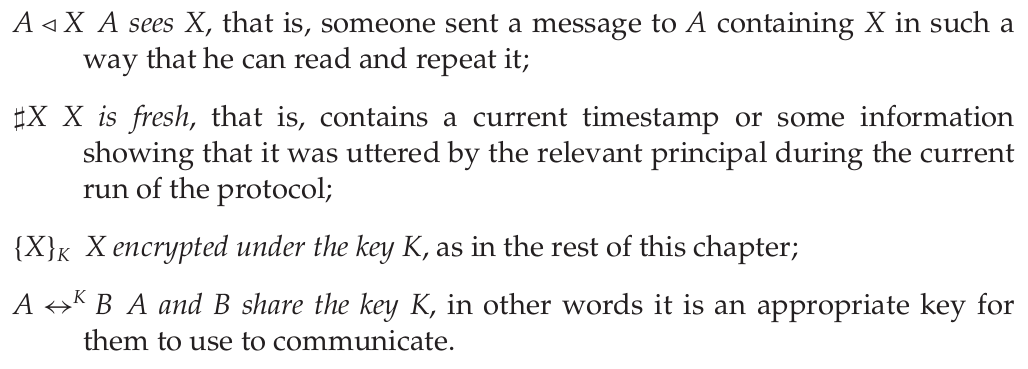
\includegraphics[scale=0.3]{pics/BAN2.png}
	\end{figure}
	\begin{figure}[H]
		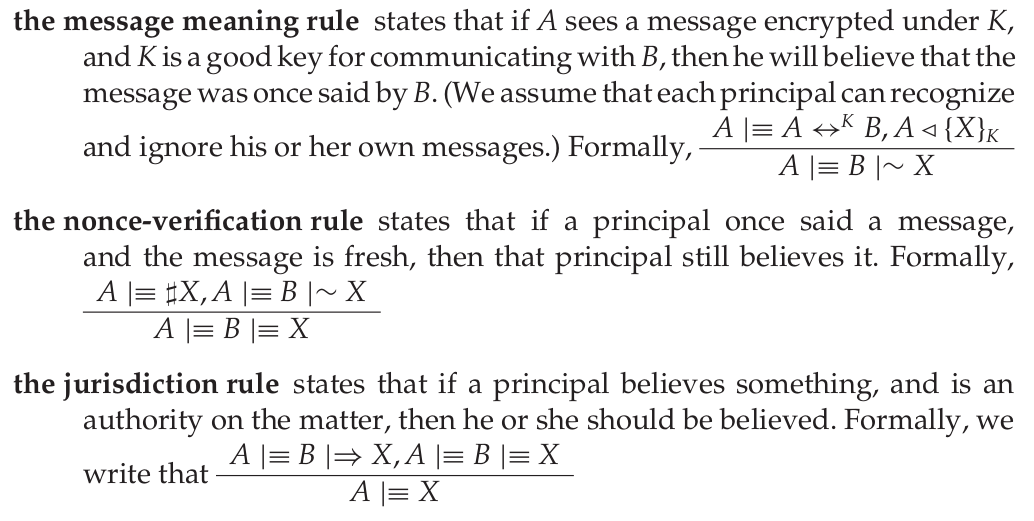
\includegraphics[scale=0.3]{pics/BAN3.png}
	\end{figure}




	\clearpage
	\chapter{Access Control}
	
	\clearpage
	Access control is the traditional center of gravity of computer security. 
	Its function is to control which principals (persons, processes, machines, . . .) 
	have access to which resources in the system — which files they can read, which 
	programs they can execute, how they share data with other principals, and so on.

	\begin{figure}[H]
		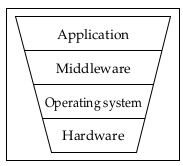
\includegraphics[scale=0.6]{pics/layers.png}
	\end{figure}

	Now one of the biggest challenges in computer security is preventing one program 
	from interfering with another. You don’t want a virus to be able to steal the 
	passwords from your browser, or to patch a banking application so as to steal 
	your money. 

	Microsoft Vista, place more emphasis on separating applications from each other; 
	even if you don’t care about security, preventing your programs from overwriting 
	each others’ configuration files should make your PC much more reliable. 

	More secure operating systems have led to ever more technical attacks on software 
	other than the operating system; you don’t want your brokerage account hacked via 
	a computer game you downloaded that later truns out to be insecure. And employers 
	would like ways of ensuring that employees’ laptops don’t pick up malware at home, 
	so it makes sense to have one partition (or virtual machine) for work and another
	for play.

	\clearpage
	\section{Operating System Access Control}

		The access controls provided with an operating system typically authenticate
		principals using a mechanism such as passwords or Kerberos, then mediate
		their access to files, communications ports and other system resources.
		Their effect can often be modelled by a {\bf matrix} of access permissions, with
		columns for files and rows for users. We’ll write {\bf r} for permission to read, 
		{\bf w} for permission to write, {\bf x} for permission to execute a program, and 
		{\bf -} for no access at all.

		\begin{figure}[H]
			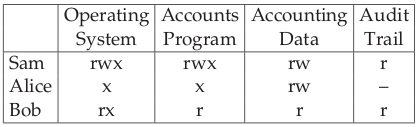
\includegraphics[scale=0.6]{pics/access1.png}
		\end{figure}

		This is often enough, but in the specific case of a bookkeeping system
		it’s not quite what we need. We want to ensure that transactions are well-
		formed — that each debit is matched by a credit somewhere else — so we
		would not want Alice to have uninhibited write access to the account file.
		We would also rather that Sam didn’t have this access. So we would prefer
		that write access to the accounting data file be possible only via the accounting
		program. 

		\begin{figure}[H]
			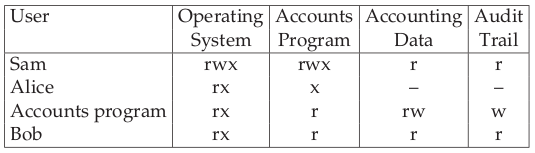
\includegraphics[scale=0.6]{pics/access2.png}
		\end{figure}

		Another way of expressing a policy of this type would be with access triples
		of (user, program, file). In the general case, our concern isn’t with a program
		so much as a protection domain which is a set of processes or threads which
		share access to the same resources.
		Access control matrices (whether in two or three dimensions) can be used to
		implement protection mechanisms as well as just model them. But they do not
		scale well. For instance, a bank with 50,000 staff and 300 applications would
		have an access control matrix of 15,000,000 entries. 

		The two main ways of doing this are to compress the users and to compress the rights. 
		As for the first of these, the 	simplest is to use groups or roles to manage the 
		privileges of {\bf large sets of users} simultaneously, while in the second we may 
		store the access control matrix
		either by {\bf columns (access control lists)} or {\bf rows (capabilities, sometimes known
		as ‘tickets’)}.

		\subsection{Groups and Roles}
			When we look at large organisations, we usually find that most staff fit into
			one or other of a small number of categories. A bank might have 40 or 50:
			teller, chief teller, branch accountant, branch manager, and so on. Only a few
			dozen people (security manager, chief foreign exchange dealer, . . .) will need
			to have their access rights defined individually.
			So we want a small number of pre-defined groups, or functional roles,
			to which staff can be assigned. 

			{\bf Group and roles:} some people use the words group and role
			interchangeably, and with many systems they are; but the more careful
			definition is that a group is a list of principals, while a role is a fixed set of
			access permissions that one or more principals may assume for a period of time
			using some defined procedure. 


		\subsection{Access Control Lists}

			Another way of simplifying the management of access rights is to store the
			access control matrix a column at a time, along with the resource to which
			the column refers. This is called an access control list or ACL (pronounced
			‘ackle’).

			\begin{figure}[H]
				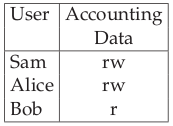
\includegraphics[scale=0.6]{pics/accessControlLists.png}
			\end{figure}

			ACLs have a number of advantages and disadvantages as a means of
			managing security state:

			\begin{itemize}
				\item ACLs are a natural choice in environments where users manage their
				own file security, and became widespread in the Unix systems. They are 
				the basic access control mechanism in Unix-based systems such as GNU/Linux and Apple’s OS/X; the access controls in Windows are also based on ACLs, 
				but have become more complex over time. 
				\item Where access control policy is set centrally, ACLs
				are suited to environments where protection is data-oriented; they are less
				suited where the user population is large and constantly changing, or where
				users want to be able to delegate their authority to run a particular program
				to another user for some set period of time. 
				\item ACLs are simple to implement, but are not efficient as a means of doing security checking at runtime.
				\item Finally, distributing the access rules into ACLs means that it can be tedious
				to find all the files to which a user has access.
			\end{itemize}

		\subsection{Unix OS Security}

			In Unix (including its popular variant Linux), files are not allowed to have
			arbitrary access control lists, but simply rwx attributes for the resource owner,
			the group, and the world. These attributes allow the file to be read, written
			and executed. The access control list as normally displayed has a flag to show
			whether the file is a directory, then flags r, w and x for world, group and owner
			respectively; it then has the owner’s name and the group name. A directory
			with all flags set would have the ACL: \\

				{\bf \color{blue} drwxrwxrwx Alice Accounts} \\


			In the example below: records that the file is not a directory; the file owner can 
			read and write it; group members can read it but not write it; non-group members have 
			no access at all; the file owner is Alice; and the group is Accounts.In our previous example, the ACL of the figure would be: \\

				{\bf \color{blue} -rw-r----- Alice Accounts} \\
				\begin{figure}[H]
					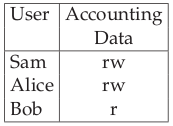
\includegraphics[scale=0.6]{pics/accessControlLists}
				\end{figure}

			In Unix, the program that gets control when the machine is booted (the
			operating system kernel) runs as the supervisor, and has unrestricted access
			to the whole machine. All other programs run as users and have their access
			mediated by the supervisor. 

			This means that (with most flavours of Unix) the system administrator can
			do anything, so we have difficulty implementing an audit trail as a file that
			he cannot modify. This not only means that, in our example, Sam could tinker
			with the accounts, and have difficulty defending himself if he were falsely
			accused of tinkering, but that a hacker who managed to become the system
			administrator could remove all evidence of his intrusion.
			Second, ACLs only contain the names of users, not of programs; so there
			is no straightforward way to implement access triples of (user, program, file).
			Third, ACLs are not very good at expressing mutable state.

		\subsection{Apple's OS/X}

			Apple’s OS/X operating system is based on the FreeBSD version of Unix run-
			ning on top of the Mach kernel. The BSD layer provides memory protection;
			applications cannot access system memory (or each others’) unless running
			with advanced permissions. At the file system level, OS/X is almost a standard Unix.


		\subsection{Windows - Basic Architecture}

			The most widespread PC operating system is Windows, whose protection
			has been largely based on access control lists. 
			
			First, rather than just read, write and execute there are separate attributes for
			take ownership, change permissions and delete, which means that more flexible
			delegation can be supported. These attributes apply to groups as well as users,
			and group permissions allow you to achieve much the same effect as suid
			programs in Unix. Attributes are not simply on or off, as in Unix, but have
			multiple values: you can set AccessDenied, AccessAllowed or SystemAudit. 

			Second, users and resources can be partitioned into domains with distinct
			administrators, and trust can be inherited between domains in one direction
			or both. 

		\clearpage
		\subsection{Capabilities}
			The next way to manage the access control matrix is to store it by rows. These
			are called capabilities. Bob’s capabilities would be:

			\begin{figure}[H]
				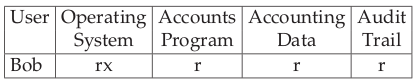
\includegraphics[scale=0.6]{pics/capabilities.png}
			\end{figure}

		The strengths and weaknesses of capabilities are more or less the opposite
		of ACLs. Runtime security checking is more efficient, and we can delegate a
		right without much difficulty. On the other hand, changing a file’s status can 
		suddenly become more tricky as it can be difficult to find out which users 
		have access. This can be tiresome when we have to investigate an incident 
		or prepare evidence of a crime.

	\section{Middleware}
		Doing access control at the level of files and programs was all very well in the
		early days of computing, when these were the resources that mattered. Since
		about the 1980s, growing scale and complexity has meant led to access control
		being done at other levels instead of (sometimes as well as) at the operating
		system level. For example, a bank’s branch bookkeeping system will typically
		run on top of a database product, and the database looks to the operating
		system as one large file. This means that the access control has to be done in
		the database; all the operating system supplies it may be an authenticated ID
		for each user who logs on.

		\subsection{Database Access Control}
			The databases now contain much of the data of greatest relevance to our lives 
			— such as bank accounts, vehicle regis-trations and employment records — 
			and front-end failures sometimes expose the database itself to random online users.
			Database products, such as Oracle, DB2 and MySQL, have their own access
			control mechanisms. As the database looks to the operating system as a single
			large file, the most the operating system can do is to identify users and to
			separate the database from other applications running on the same machine.

		\subsection{General Middleware Issues}
			There are a number of aspects common to middleware security and application-
			level controls. The first is {\bf granularity:} as the operating system works 
			with files, these are usually the smallest objects with which its access control mechanisms can deal. The second is {\bf state}. An access rule such as ‘a nurse can 
			see the records of any patient on her ward’ or ‘a transaction over \$100,000 
			must be authorised by a manager and an accountant’ both involve managing state.
			The third is {\bf level:} we may end up with separate access control systems at 
			the machine, network and application levels, and as these typically come from 
			different vendors it may be difficult to keep them consistent.


			Ease of administration is often a critical bottleneck. In companies the 
			administration of the operating system and the database system
			have been done by different departments, which do not talk to each other;
			and often user pressure drives IT departments to put in crude hacks which
			make the various access control systems seem to work as one, but which open
			up serious holes. An example is ‘single sign-on’. 

			Despite the best efforts of computer managers, most large companies accumulate 
			systems of many different architectures, so users get more and more logons to 
			different systems and the cost of administering them escalates. 
			Many organisations want to give
			each employee a single logon to all the machines on the network. 
			Commercial solutions may involve a single security server through which all 
			logons must pass, and the use of a smartcard to do multiple authentication 
			protocols for different systems. Such solutions are hard to engineer properly, 
			and the security of the best system can very easily be reduced to that of the worst.

		\subsection{ORBs and Policy Languages}
			Problems with middleware led researchers to look for ways in which access control 
			for a number of applications might be handled by standard middleware. Research
			in the 1990s focussed on object request brokers (ORBs). An ORB is a software
			component that mediates communications between objects.
			An ORB typically provides a means of controlling calls that are made across 
			protection domains. The Common Object Request Broker Architecture (CORBA) is an 
			attempt at an industry standard for object-oriented system.

			Languages to express security policy, with projects such as XACML (Sun), XrML 
			(ISO) and SecPAL (Microsoft).

		\subsection{Sandboxing and Proof-Carrying Code}
			The late 1990s saw the emergence of yet another way of implementing access
			control: the software {\bf sandbox}. 
			The model is that a user wants to run some code that she has downloaded 
			from the web as an applet, but is concerned that
			the applet might do something nasty, such as taking a list of all her files and
			mailing it off to a software marketing company.
			The designers of Java tackled this problem by providing a ‘sandbox’ for such
			code — a restricted environment in which it has no access to the local hard
			disk, and is only allowed to communicate with the host it came from.

			An alternative is {\bf proof-carrying code}. Here, code to be executed must carry
			with it a proof that it doesn’t do anything that contravenes the local security
			policy. This way, rather than using an interpreter with the resulting speed
			penalty, one merely has to trust a short program that checks the proofs
			supplied by downloaded programs before allowing them to be executed.

		\subsection{Trusted Computing}
			The ‘Trusted Computing’ initiative was launched by Microsoft, Intel, IBM, HP
			and Compaq to provide a more secure PC. Their stated aim was to provide
			software and hardware add-ons to the PC architecture that would enable
			people to be sure that a given program was running on a machine with a
			given specification; that is, that software had not been patched (whether by
			the user or by other software) and was running on a identifiable type and
			configuration of PC rather than on an emulator. The initial motivation was
			to support digital rights management.


	\clearpage
	\section{Hardware Protection}
		--Write something?--






	\clearpage
	\chapter{Cryptography}
	\clearpage
	\chapter{Multilevel Security}
	\clearpage
	\chapter{Multilateral Security}

\end{document}